\documentclass[9pt,twocolumn]{extarticle}

\usepackage[hmargin=0.5in,tmargin=0.5in]{geometry}
\usepackage{amsmath,amssymb,subfigure,graphicx}
\usepackage{times}

\usepackage{cleveref}
\usepackage{color}
\newcommand{\TODO}[1]{\textcolor{red}{#1}}

\newcommand{\FPP}[2]{\frac{\partial #1}{\partial #2}}
\newcommand{\argmin}{\operatornamewithlimits{arg\ min}}

\title{Experiments with unconstrained animation}
\author{Siwang Li}

\begin{document}
\maketitle

\setlength{\parskip}{0.5ex}

\section{Setup}
The input animation $u_1,\cdots,u_{100}$ is \TODO{unconstrained}, and it is
generated using a RS simulator \TODO{without external forces}, with time step
$h=0.1$. To produce such an animation, we firstly project a deformed shape $u_0$
to obtain the initial state $z_0$ in subspace using RS-coordinates, then
integrate the motion equation to obtain the whole animation
$z_1,\cdots,z_{100}$, and finally recover $u_1,\cdots,u_{100}$ by using RS
method with the barycenter are fixed. The input animation can be found in the
attached video.

In the following experiments, we use $r=10$ modes, and the first $6$ modes are
rigid modes, and the corresponding correct eigenvalues are $(-9\times
10^{-13},-1\times 10^{-13},-9\times 10^{-14},3\times 10^{-14},2\times
10^{-13},3\times 10^{-13},\TODO{1.519,5.727,11.88, 20.37})$. We also use a
correct basis $\hat{W}$ to obtain $z'_i=\hat{W}^{-p}y'_i$ for frame $i$, where
$y'_i=T(u_i)$, and $T(\cdot)$ is the mapping function that is used to compute
the RS coordinates.

Given $z_i$ or $z'_i$, we minimize a quadratic energy function to obtain
$p=(d^T,k^T)^T$,
\begin{equation} \label{qua-en}
  E(p) = \sum_{i=2}^{T-1} \|\frac{1}{h^2}\hat{z}_i+\frac{1}{h}{D}(d)(z_{i+1}-z_{i})+ K(k)z_i\|_2^2
\end{equation}
which is equal to solve
\begin{equation} \label{leq}
  Hp + b = 0
\end{equation}
where $H$ and $b$ are constant, and $H=\frac{\partial^2{E}}{\partial^2{p}}$.  In
the following, we will analysis the conditional number for $H$.

\section{Experiments}
In the first experiment, we compare results with and without rigid modes using
the \TODO{correct} reduced displacement $z_0,\cdots,z_{100}$.  When all rigid
modes are used, the eigenvalues are
$(\TODO{0.00024,1.527,7.133,13.08,29.32,73.09,78.3,90.5,105.97,140.3})$, and the
conditional number of $H$ is $cond(H)=\|H\|\|H^{-1}\|=\TODO{7.3\times
  10^{8}}$. When rigid modes are removed from $z_i$, e.g use the bottom $4$ rows
in $Z=(z_0,\cdots,z_{100})$ for approximation, then the eigenvalues are
$(\TODO{1.520, 5.727, 11.88, 20.37})$, and $cond(H)=\TODO{8.2\times 10^{5}}$.

In the second experiment, we found that, if we scale each modes, e.g normalize
the rows in $Z=(z_0,\cdots,z_{100})$, the conditional number of $H$ will be much
better. After removing the rigid modes, and scale the remaining modes, we obtain
$cond(H)=\TODO{128.4}$, and the eigenvalues are $(1.520,5.727,11.88,20.37)$.

In the third experiment, we check the difference between the recovered RS
coordinates $y'_i=T(u_i)$ and the correct values $y_i=\hat{W}z_i$ and we found
that $\|y'_i-y_i\|$ is large and almost the same for all frames $i$. This is not
because of inverted tetrahedrons, and much like a difference in the global
rotation.

In the fourth experiment, we draw the curves of the first 9 modes of $z_i$ and
$z'_i$ in figure \ref{dft}. The difference in $y'$ results in the difference in
$z'_i$. However, in first non-rigid mode (mode 7), they are similar.

\begin{figure}
  \centering
  \subfigure[mode 1,2,3] { \label{fig:a}
    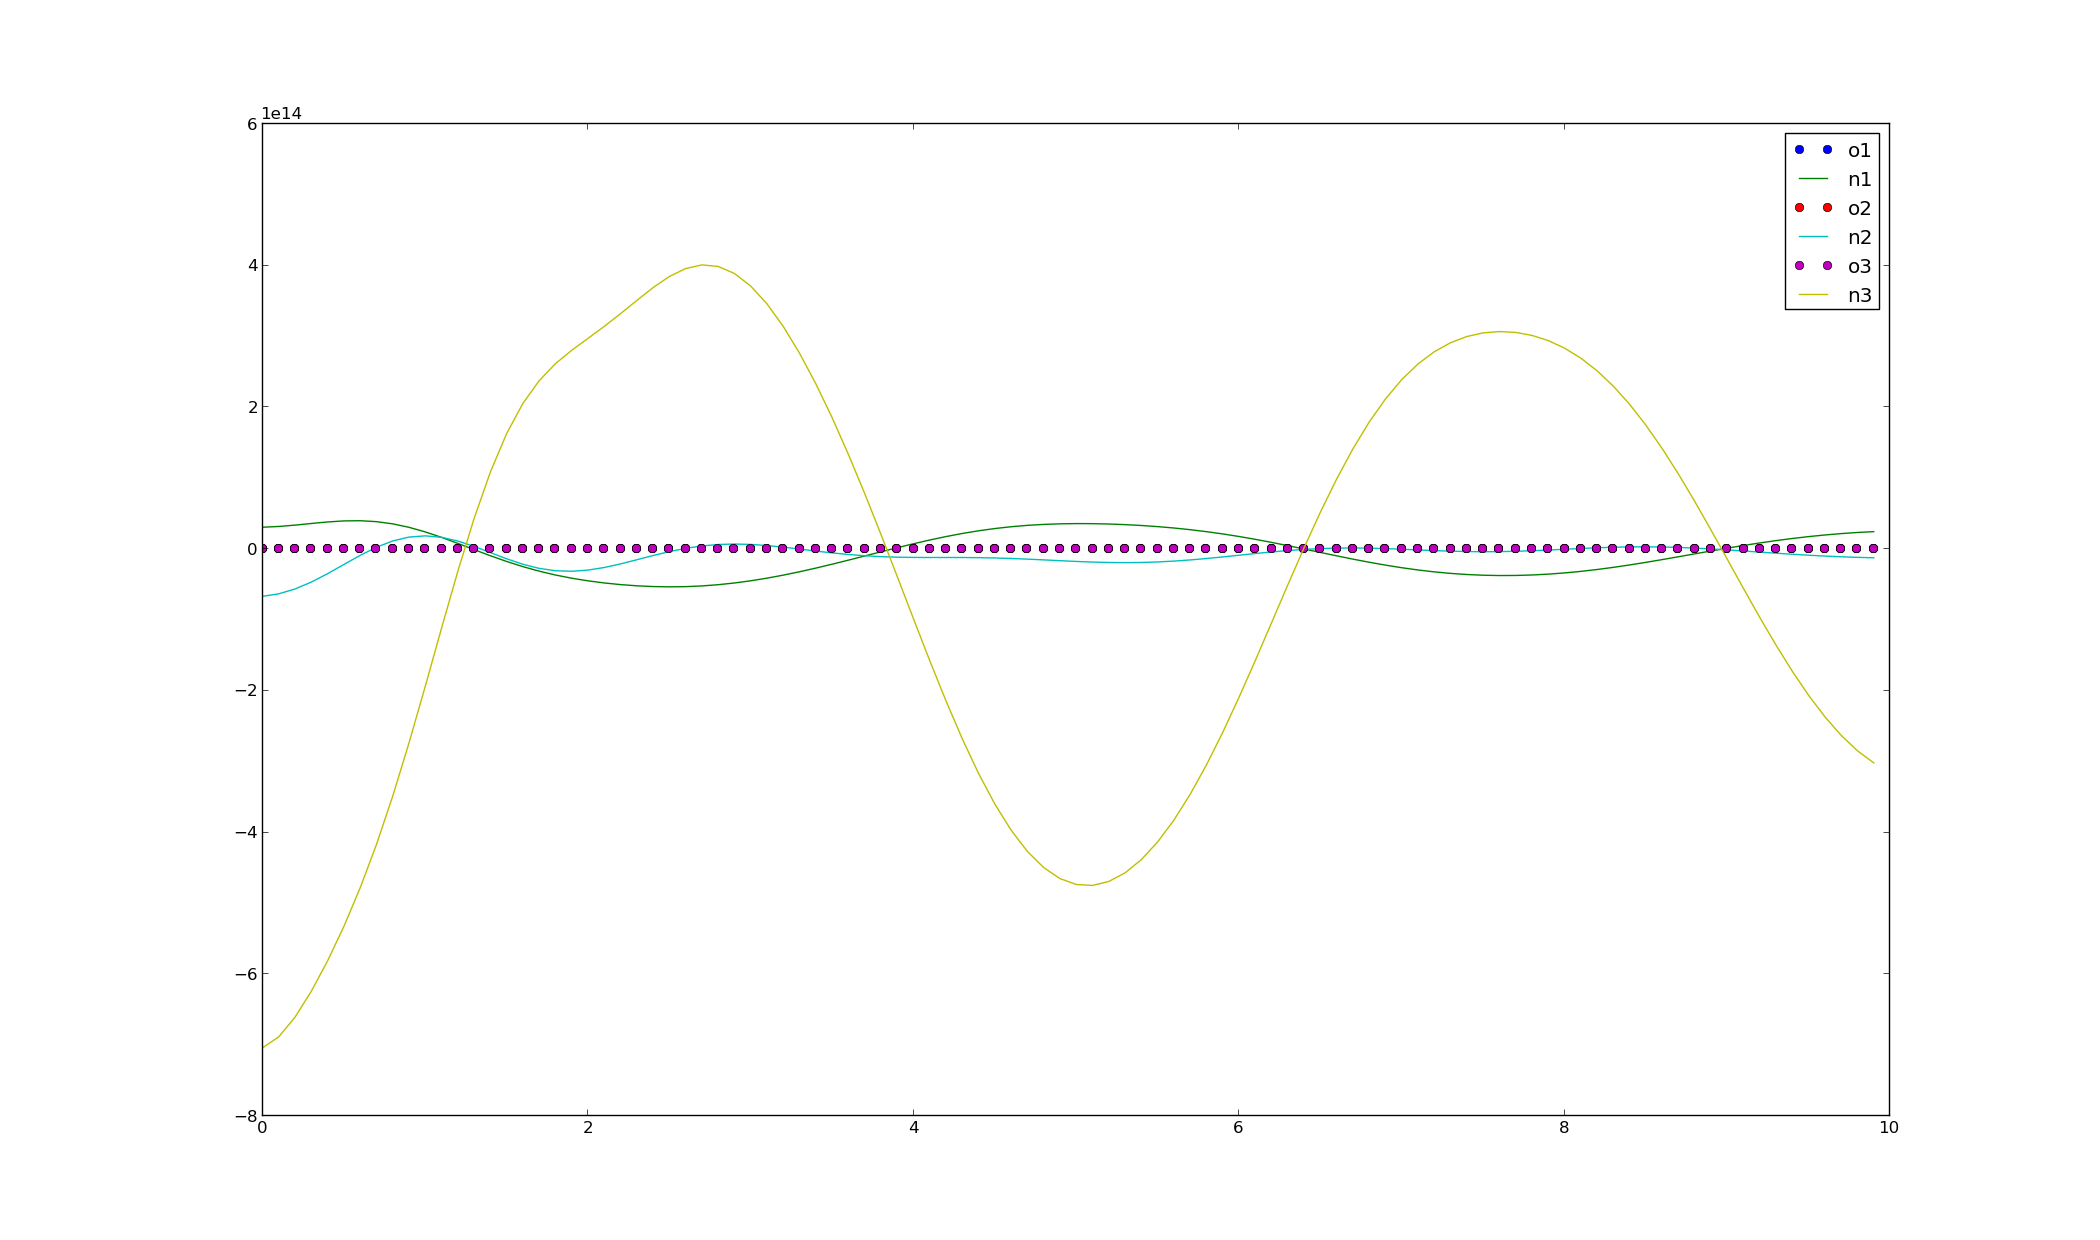
\includegraphics[width=0.48\textwidth]{./figures/noncon1-3.png}
  }
  \subfigure[mode 4,5,6] { \label{fig:b} 
    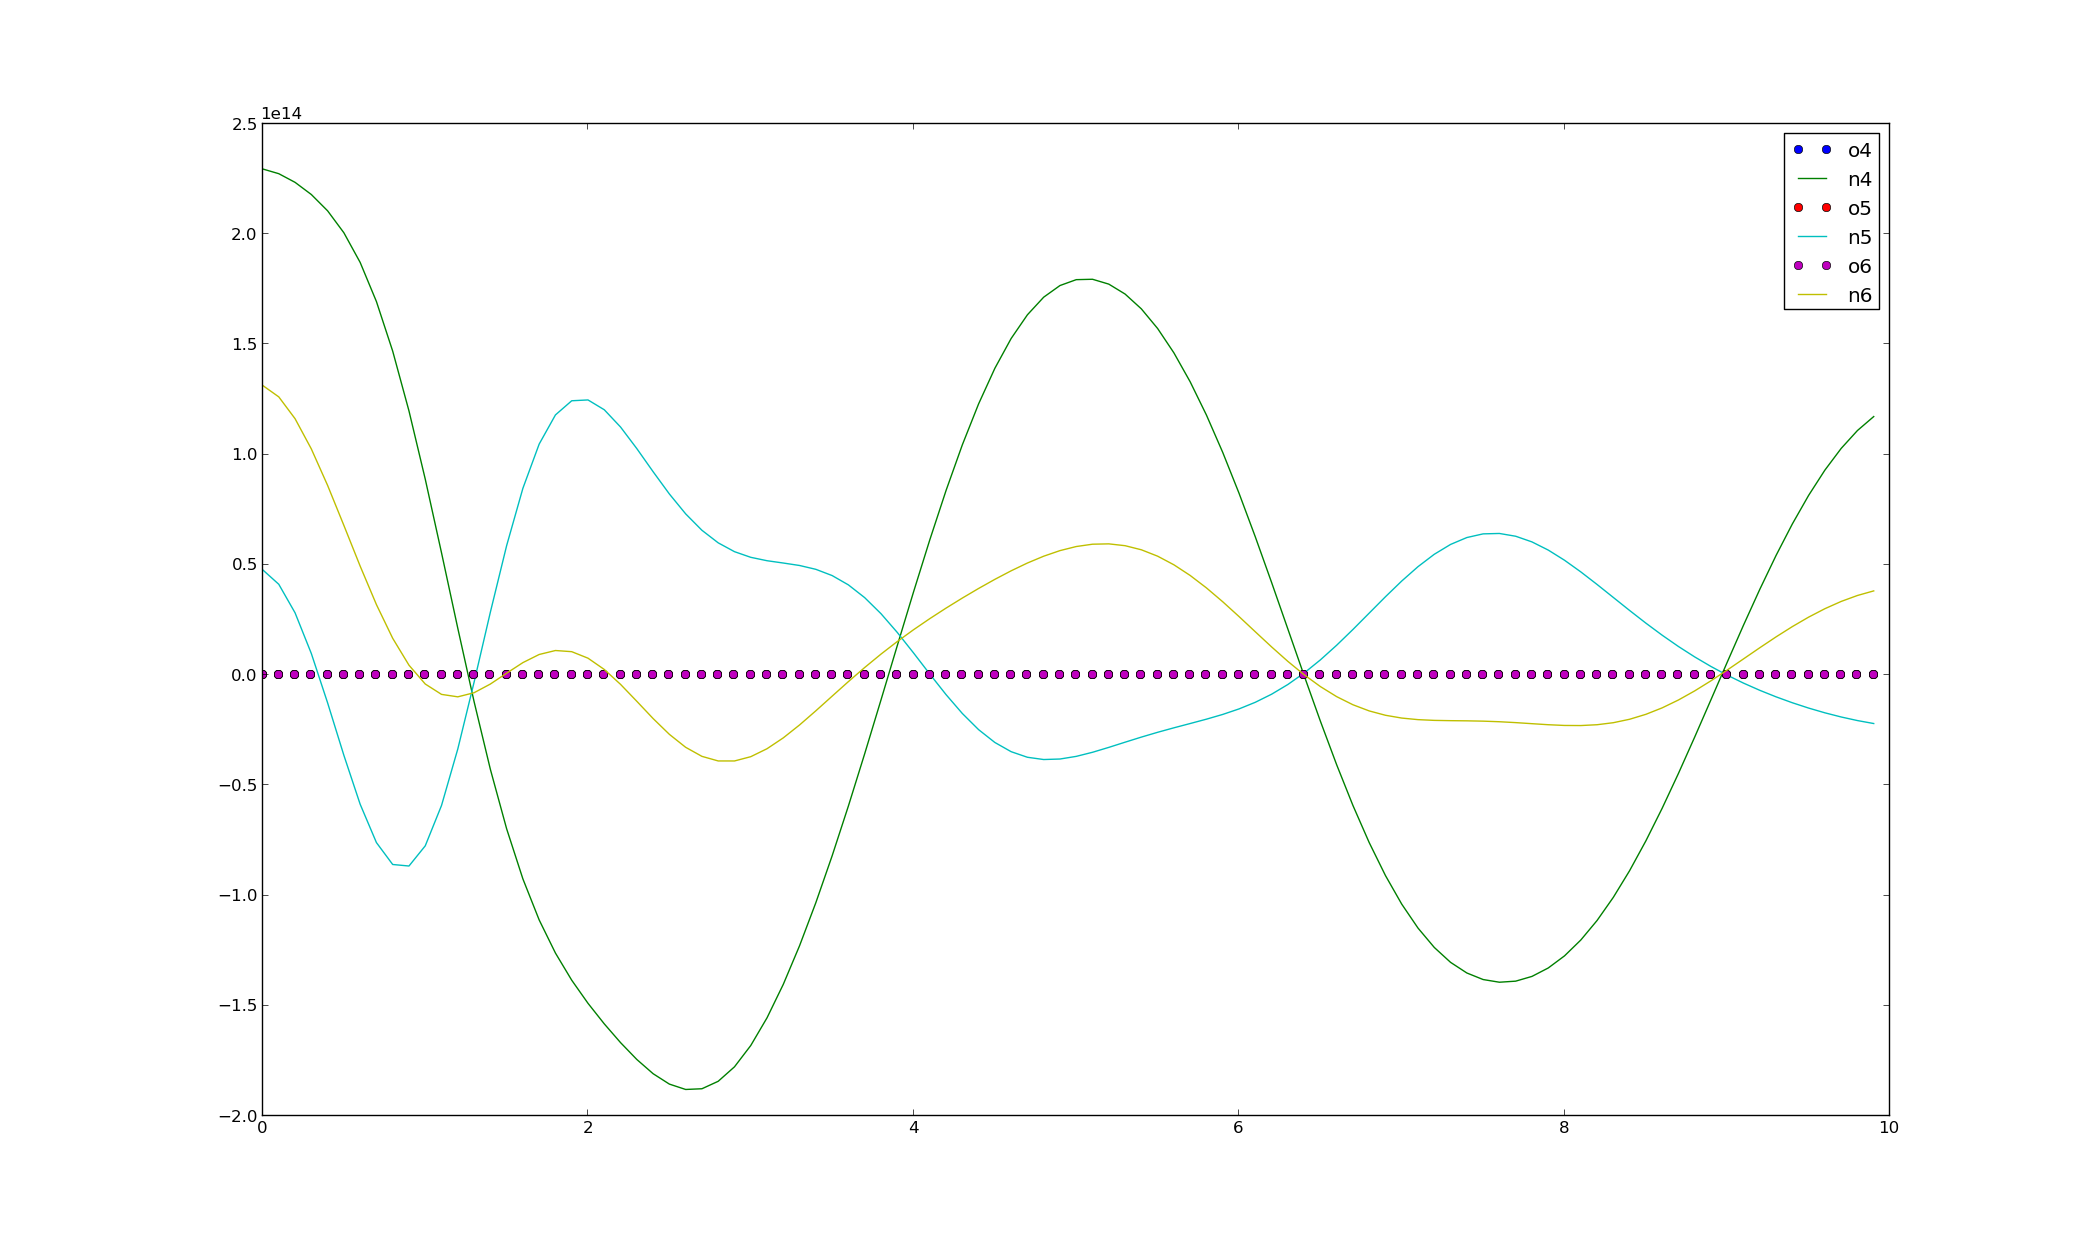
\includegraphics[width=0.48\textwidth]{./figures/noncon4-6.png}
  }
  \subfigure[mode 7,8,9] { \label{fig:b} 
    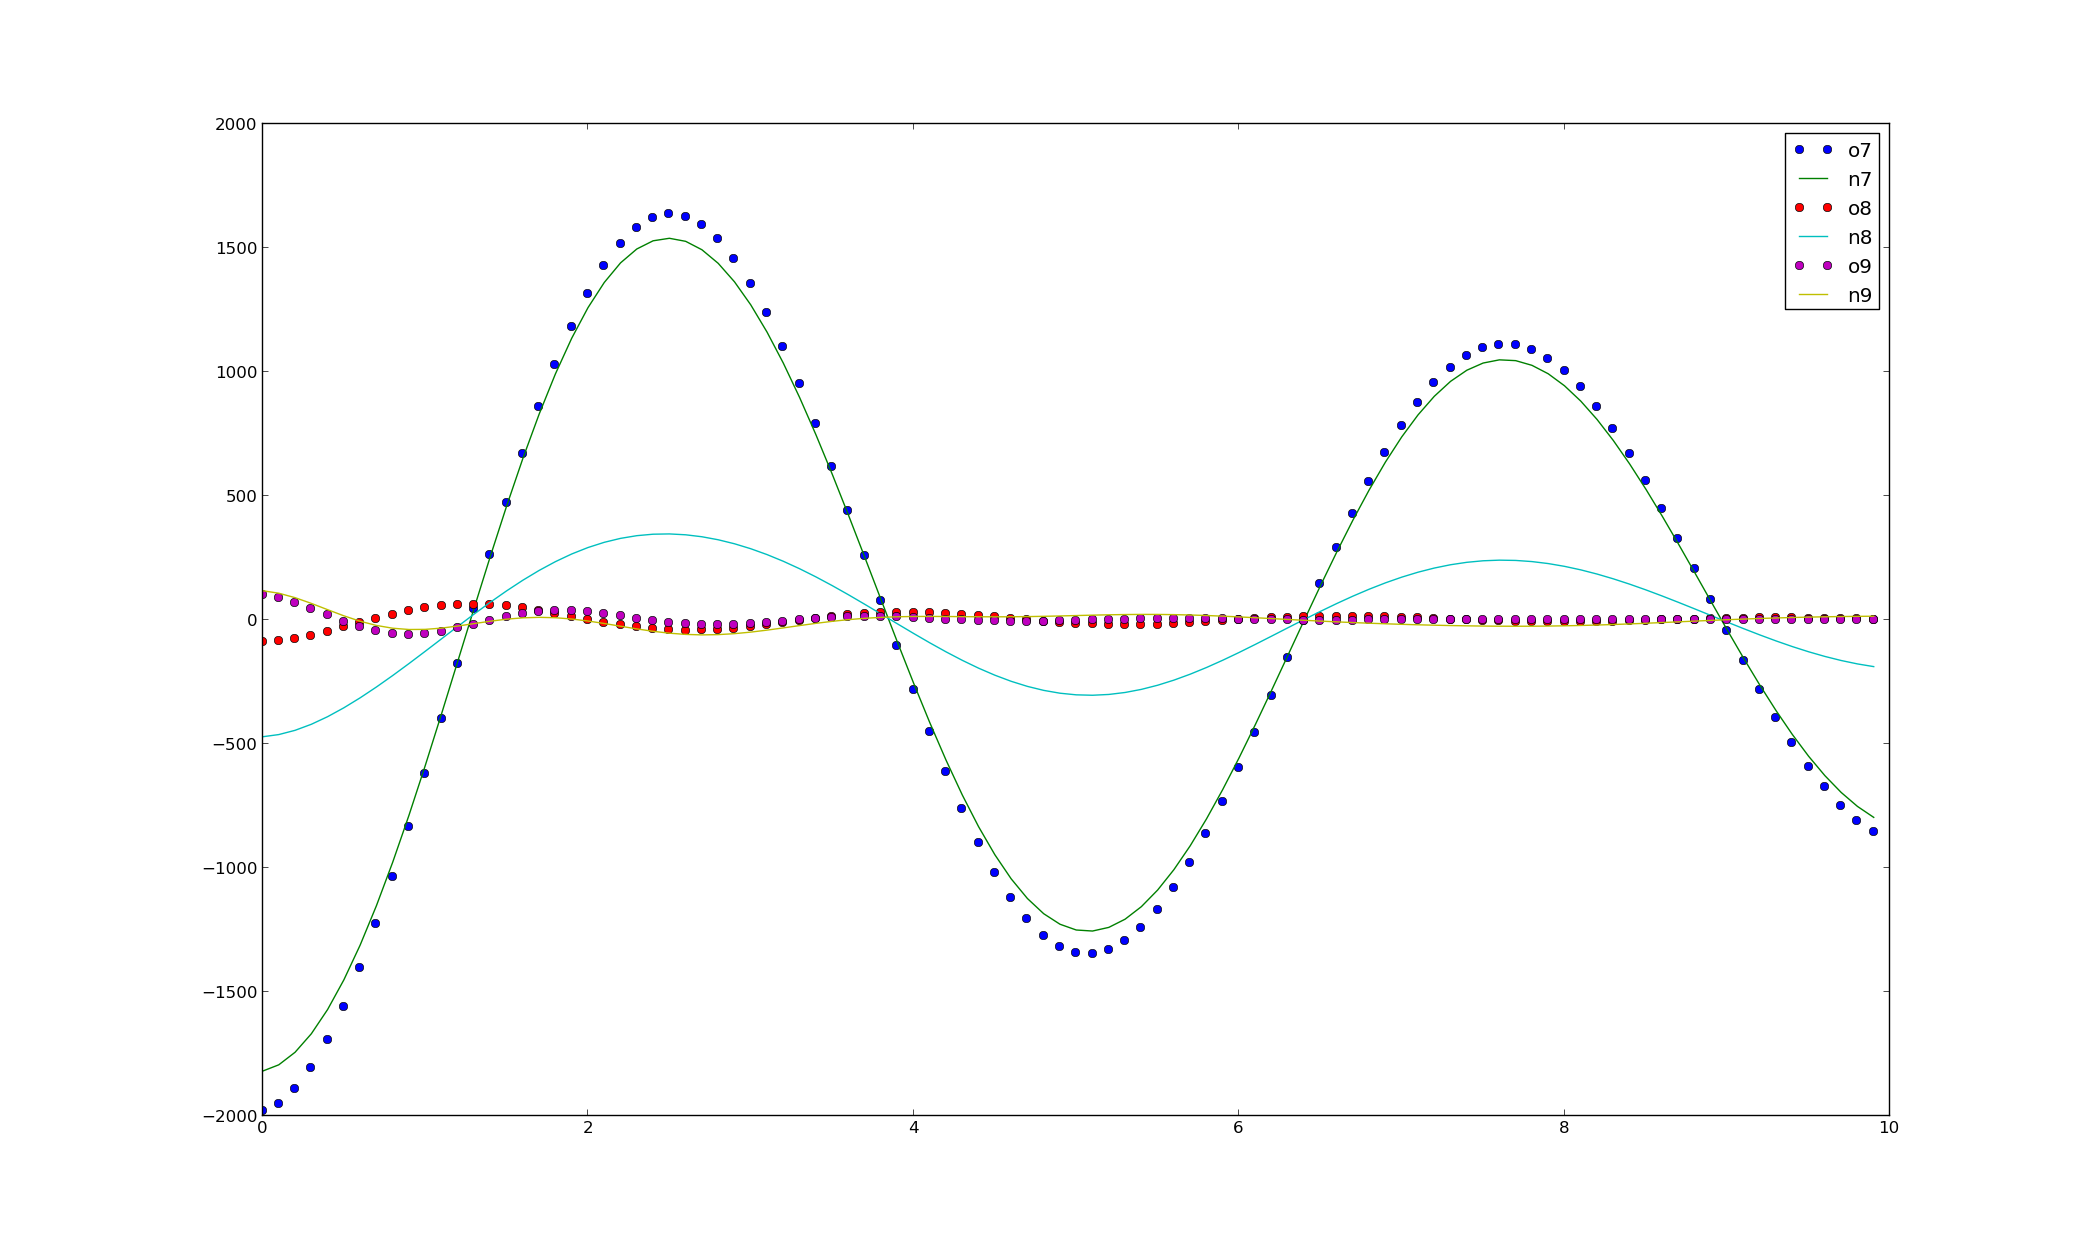
\includegraphics[width=0.48\textwidth]{./figures/noncon7-9.png}
  }
  \caption{The curves of each mode of the recovered reduced coordinates
    $z'$(solid) and the correct $z$(in points). The motion are dominated by mode
    7, and $z'$ and $z$ are only similar at this mode. The motion of each mode
    in $z$ can also be found in the attached video.}
  \label{dft}
\end{figure}

In the final experiment, we use $z'_i$ to approximate the material with and
without rigid modes. When rigid modes are considered, we found
$cond(H)=\TODO{8.4\times 10^{30}}$, and failed to solve for $k,d$. And when the
rigid modes are removed, $cond(H)=8.97\times 10^6$, and we success to
approximate the eigenvalues $(\TODO{1.522,4.010,11.31,15.69})$.

\section{Conclusion}
\begin{itemize}
\item The rigid modes will significantly impact the approximation. It will
  result large conditional number of $H$, and produce incorrect results. We can
  truncate these rigid modes from the reduced coordinates to solve this problem.
\item The motion on some modes are much larger than others, and it is much
  easier to recover the material for these modes than others. For example, in
  this experiment, the amplitude of mode $7$ are much larger than others, and
  the material approximation result of this mode are much better.
\item When the input animation is not constrained, $\|y'_i-y_i\|$ is large and
  almost the same for all frames $i$. The difference is from the rotational part
  of $y$. As a result, the difference between $z'_i=\hat{W}^{-p}y'_i$ and $z_i$
  are also very large, except the $7$-th mode.
\item The conditional number of $H$ is usually very large even there is no rigid
  modes. This is because the amplitude in $z_i$ of each mode differs greatly,
  e.g, some are very large, and others are very small. In this experiment, as
  the modes in $z_i$ are decoupled, we can solve this problem by scaling the
  motion for each mode. But in the general case, when the modes in $z_i$ are
  coupled, it is non-trivial.
\end{itemize}


\end{document}